\pagestyle{empty}
\begin{center}
	{\Large {\textbf{外文资料原文}}}
\end{center}
\begin{figure}[h]
	\centering
	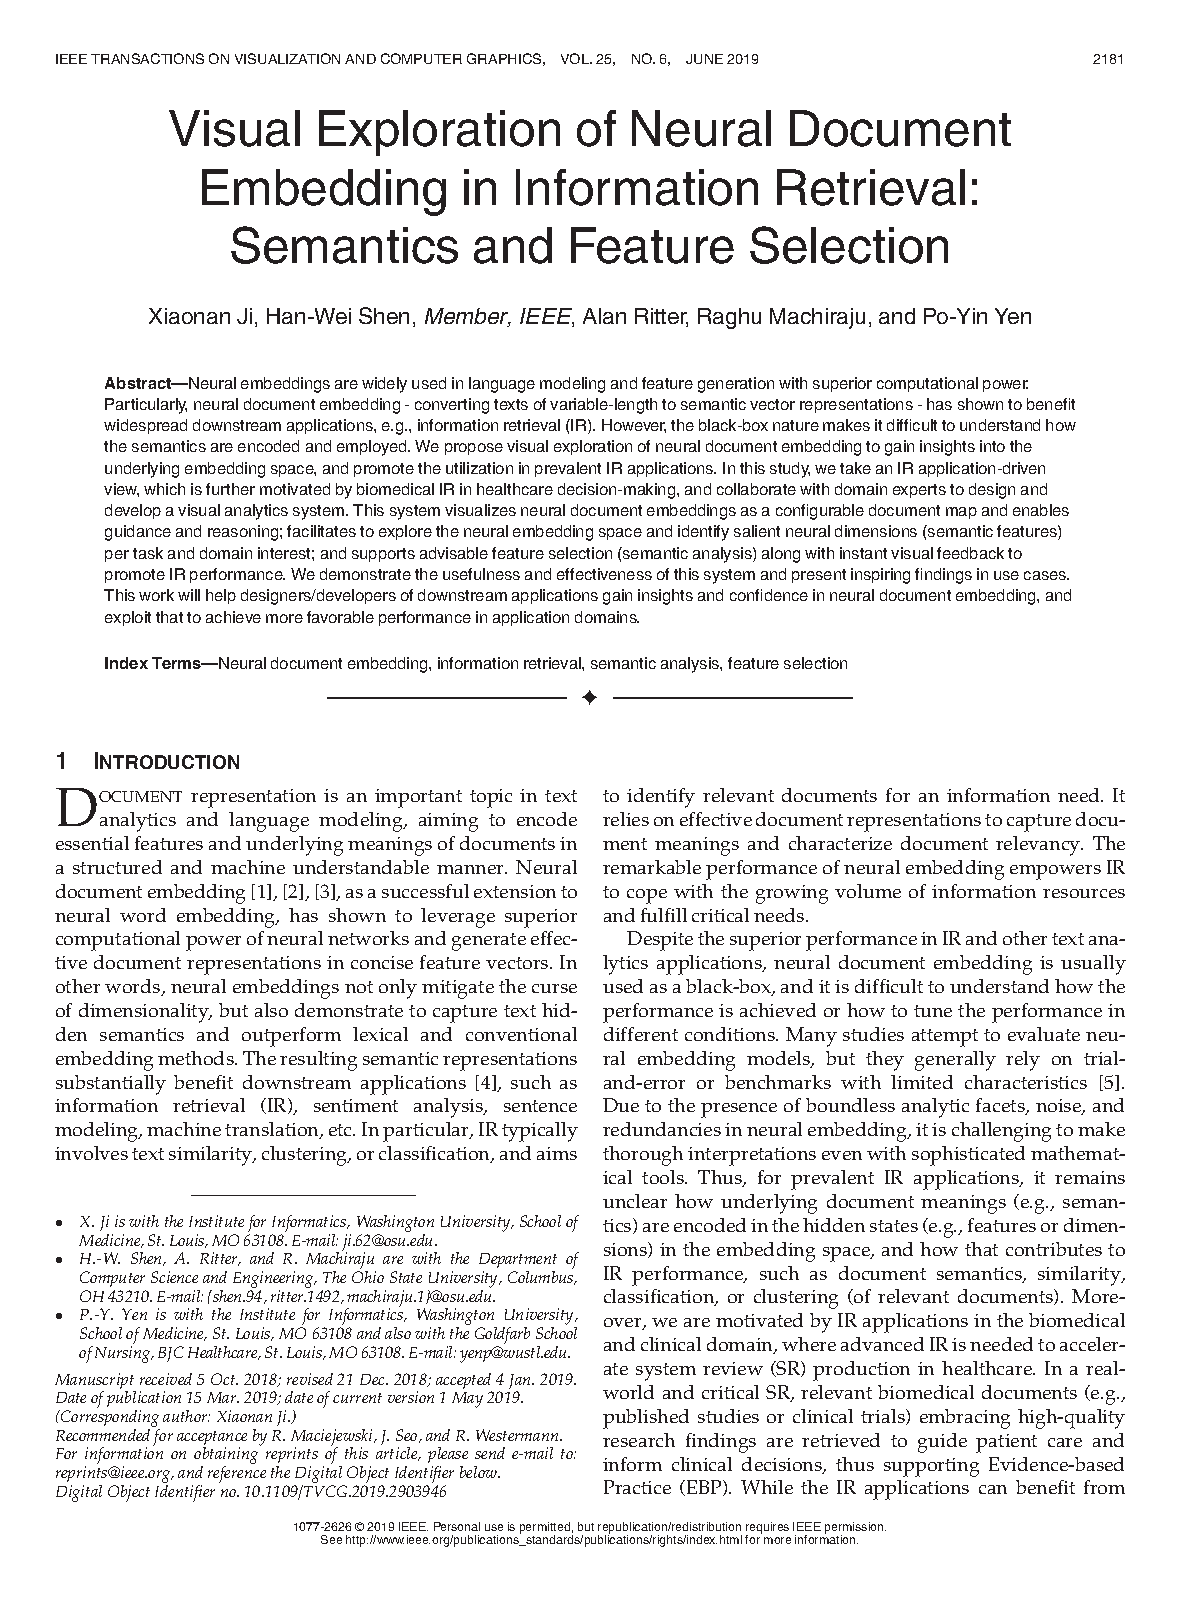
\includegraphics[height=0.77\textheight]{trans}
	\label{pic-trans}
\end{figure}

\newpage
\begin{center}
	{\Large {\textbf{信息检索中神经文档嵌入的可视化探索:语义与特征选择}}}
\end{center}
\begin{center}
	{\large {\textbf{Xiaonan Ji, Han-Wei Shen, Member, IEEE, Alan Ritter, Raghu Machiraju, and Po-Yin Yen}}}
\end{center}

\textbf{摘要}——神经嵌入广泛应用于语言建模和特征生成,具有卓越的计算能力。特别地,神经文档嵌入 将可变长度的文本转换为语义向量表示,已经显示出有益于广泛的下游应用,例如信息检索(IR)。然而,黑盒性质使得难以理解语义是如何被编码和使用的。我们提出了神经文档嵌入的可视化探索,以深入了解底层嵌入空间,并促进在流行的IR应用中的使用。在本研究中,我们采用IR应用驱动的观点,该观点由医疗保健决策中的生物医学IR进一步推动,并与领域专家合作设计和开发可视化分析系统。该系统将神经文档嵌入可视化为可配置的文档图,并实现指导和推理;有助于探索神经嵌入空间并识别每个任务和领域兴趣的突出神经维度(语义特征),并支持可行的特征选择(语义分析)以及即时视觉反馈以促进IR性能。我们展示了该系统的有用性和有效性,并在用例中展示了令人鼓舞的发现。这项工作将帮助下游应用程序的设计人员/开发人员获得神经文档嵌入的见解和信心,并利用它来在应用程序域中实现更好的性能。
索引术语——神经文档嵌入,信息检索,语义分析,特征选择

\textbf{1 介绍}

文档表示是文本中的一个重要主题。分析和语言建模,旨在以结构化和机器可理解的方式编码文档的基本特征和基本含义。神经文档嵌入[1],[2],[3]作为神经词嵌入的成功扩展,已经证明可以利用神经网络的卓越计算能力,并在简洁的特征向量中生成有效的文档表示。换句话说,神经嵌入不仅减轻了维度的诅咒,而且还证明了捕获文本隐藏语义并且优于词法和常规嵌入方法。由此产生的语义表示大大有益于下游应用[4],如信息检索(IR),情感分析,句子建模,机器翻译等。特别是,IR通常涉及文本相似性,聚类或分类,旨在识别相关有关信息需求的文件。它依赖于有效的文档表示来捕获文档含义并表征文档的相关性。神经嵌入的卓越表现赋予了IR应对不断增长的信息资源并满足关键需求。尽管在IR和其他文本分析应用程序中具有优越的性能,但神经文档嵌入通常用作黑盒子,并且很难理解如何实现性能或如何在不同条件下调整性能。许多研究试图评估神经嵌入模型,但它们通常依赖于具有有限特征的试错法或基准[5]。由于神经嵌入中存在无限的分析方面,噪声和冗余,即使使用复杂的数学工具也需要进行全面的解释。因此,对于普遍的IR应用,仍然不清楚底层文档的含义(例如,语义)如何在嵌入空间中的隐藏状态(例如,特征或维度)中编码,以及它如何有助于IR性能,例如文档语义,相似性,分类或聚类(相关文档)。此外,我们的动机是生物医学和临床领域的IR应用,其中需要先进的IR来加速医疗保健中的系统评估(SR)生产。在真实的世界和关键的SR中,检索包含高质量研究结果的相关生物医学文献(例如,已发表的研究或临床试验)以指导患者护理并为临床决策提供信息,从而支持基于证据的实践(EBP)。虽然IR应用程序可以受益于有利的神经文档嵌入,但仍然不清楚域和任务感兴趣的语义如生物医学概念和主题如何在神经嵌入中编码和构建。
因此,我们使用可视化分析来探索具有两个主要目标的神经文档嵌入:(1)理解潜在的机制,特别是如何在神经维度中编码语义(例如,隐藏的语义特征),以及(2)与解释,应用通过每个域或任务兴趣的特征选择(语义分析)来增强IR性能的适当配置。为了实现上述目标,我们采用应用驱动的观点,并与在医疗保健领域培养(即设计和开发)IR应用的领域专家合作。然后,我们制定一系列可视化分析任务,并迭代开发可视化分析系统。我们的工作还受以下因素的启发:1)神经模型的可视化分析,以阐明神经元行为学习特征或表征之间的关系,以及相关的表现和2)文档语料库的可视化分析,以揭示文档特征,表示的可解释属性和模式,和关系,从而促进探索。在不同类型的神经文档嵌入模型中,我们使用段落矢量(PV)模型[1],这是一个在IR中证明有效的通用模型。我们的研究设计可推广用于记录由其他模型产生的嵌入,例如卷积神经网络(CNN)和递归神经网络(RNN)。总之,我们的工作有助于:
启用神经文档嵌入的探索和解释,特别是关于域和任务兴趣的编码语义。
促进嵌入空间中的语义特征选择,以提高IR应用程序的性能。
验证有用且有效的可视化分析系统,使用用例来增强人工解释和利用神经文档嵌入。
将视觉文本分析应用于紧迫的现实问题,即医疗保健中的生物医学IR和SR / EBP。